

\title{New plots: chapter on varrying IR}
\author{
        Chris McWilliams*, Alan Champneys, Miguel Lurgi,\\ Jose Montoya, Daniel Montoya \\ \\
				*Bristol Centre for Complexity Sciences, University of Bristol.\\
                chris.mcwilliams@bristol.ac.uk\\
}
\date{\today}

\documentclass[12pt]{article}
\usepackage{mathtools}
\usepackage{amsmath}
\usepackage{amssymb}
\usepackage{appendix}
\usepackage{graphicx}
\usepackage{caption}
\usepackage{subcaption}
\usepackage{rotating}
%\usepackage{subfig}
\usepackage[font={small,it}]{caption}
\usepackage[font={small,it}]{subcaption}
\usepackage{todo}
\setlength\parindent{0pt}
\setlength{\parskip}{10pt plus 1pt minus 1pt}

\newcommand{\mbeq}{\overset{!}{=}}

\begin{document}
\maketitle
\newpage


\subsection{Estimator comparison}
\label{sec:estimators}
%% This figure produce by: /MyFiles/cm1788/Documents/IM_vs_HL_heatmap/clean_results/random/plot_pval.py
\begin{figure}
	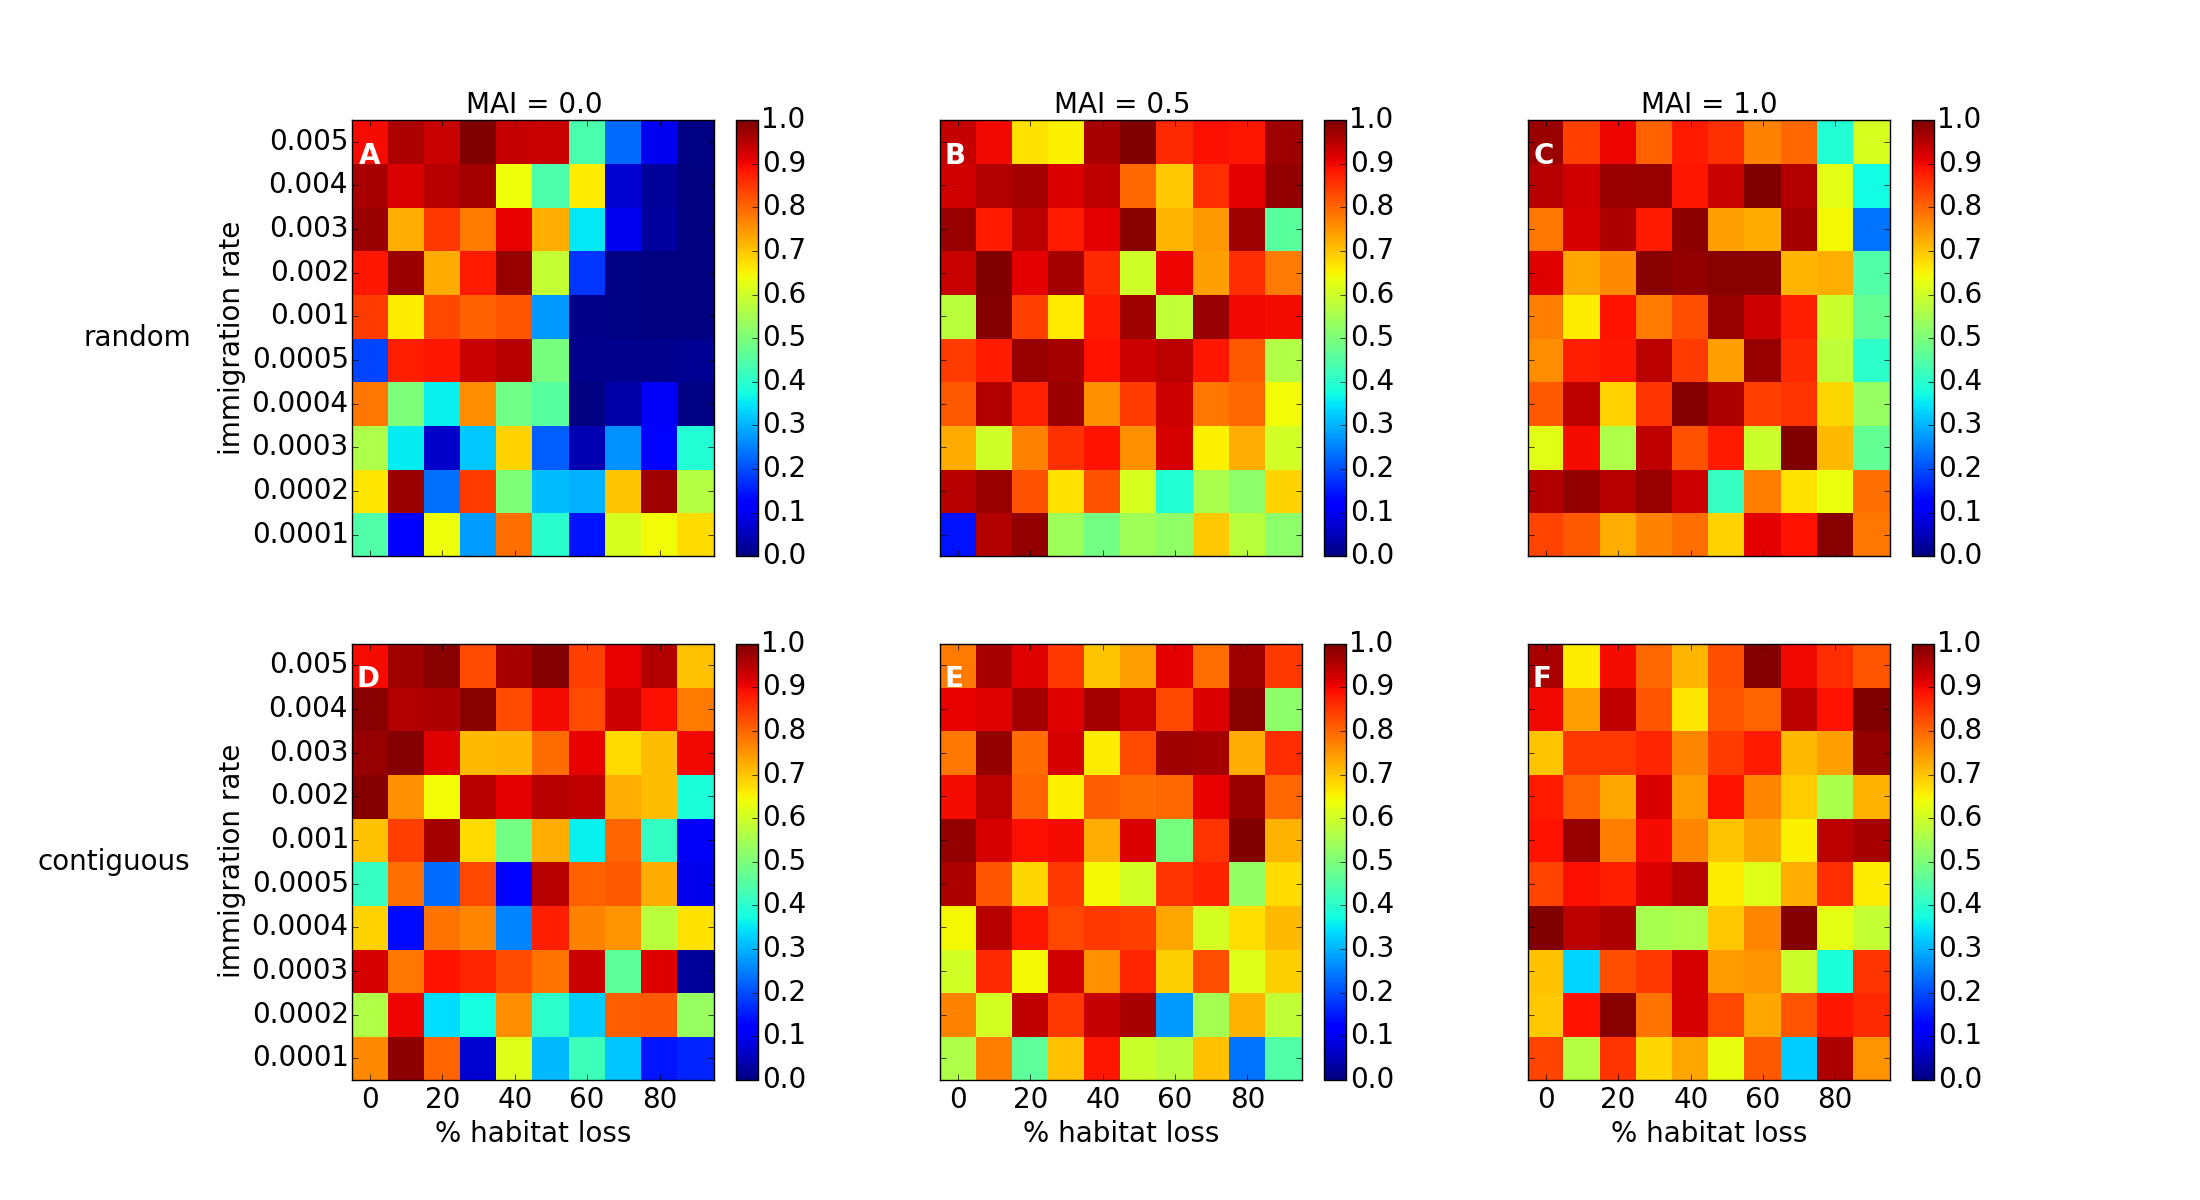
\includegraphics[width=\textwidth]{{{../figures/clean_analysis/heatmap_ttest}}}
	\caption{P-values for t-tests to compare the \emph{Shannon equitability} calculated by two different sampling methods: \emph{snapshot} and \emph{averaged} sampling (see text for definitions). Each point in the plot represents the p-value of the test comparing the \emph{snapshot} and \emph{averaged} Shannon equitability results for the 50 replicate simulations at the corresponding HL and IR value. A p-value$<0.05$ (i.e.dark blue) represents $95\%$ confidence that the two sampling methods produce different average equitability results.}
	\label{fig:ttest}
\end{figure}

The \emph{Shannon equitability} metric (equation \eqref{eq:shan_eq}) is calculated for all simulations using two different sampling methods. The first method uses snapshot sampling (as in chapter \ref{chap:}) i.e. species abundances are measured on the last time step of the simulation. The second method takes the mean species abundance over the final 4000 time steps of the simulation. Results obtained using the two sampling methods are referred to as \emph{snapshot} and \emph{averaged}, correspondingly. We compare the results obtained using a \emph{two-sided t-test}, which is implemented in the \emph{Python} package \emph{scipy}. The test is used to compare two datasets of independent samples, testing the null hypothesis that the expected value of the two datasets are equal. If the \emph{p-value} of the test is smaller than the confidence threshold then there is sufficient evidence to reject the null hypothesis and conclude that the means of the two datasets are significantly different. For each test we are comparing the \emph{snapshot} and \emph{averaged} equitability results, calculated from the 50 replicate simulations at a given HL and IR value. If the test is significant then we conclude that the two sampling methods give significantly different average results at that value of HL and IR. We conduct tests for all HL and IR values, and all three MAI ratios, under random and contiguous HL. The \emph{p-values} of these tests are depicted in figure \ref{fig:ttest}.  

In general figure \ref{fig:ttest} shows that there is strong support for the conclusion that the two sampling methods produce the same average equitability results. The worst case is random HL at MAI$=0.0$ (panel A). In this case there is a region of parameter space, above HL$=60\%$, where the p-values are significant. Therefore in this region the methods appear to give statistically different results. However, as stated, most of the tests suggest that the two methods produce statistically similar results. The similarity between the two methods is surprising given the results of the estimator analysis in section \ref{sec:convergence}. Presumably averaging over 50 replicate simulations provides some reduction in noise. It may also be that a high level of precision in the estimates of species abundances is not required to calculate community level metrics. Based on the comparison presented here we conclude that snapshot sampling is sufficient to draw general conclusions about community structure over the ensemble of simulations. This allows consistency with the analysis in chapter \ref{chap:habitat_loss_high_immigration}. However we acknowledge that the use of snapshot samples may introduce some error, and increased variability, into our calculations. We treat the region of parameter space in which the equitability results proved dissimilar (panel A: random HL. MAI$=0.0$) with particular caution.

%
%\section{Extinctions, Abundance, Diversity}
%%\clearpage
%\begin{figure}[hb]
%	\includegraphics[width=\textwidth]{{{../figures/clean_analysis/random/heatmap1}}}
%	\caption{Random HL. Number of extinctions, total number of individuals and diversity (Shannon eq.)}
%\end{figure}
%
%\begin{figure}[hb]
%	\includegraphics[width=\textwidth]{{{../figures/clean_analysis/contiguous/heatmap1}}}
%	\caption{Contiguous HL. Number of extinctions, total number of individuals and diversity (Shannon eq.)}
%\end{figure}
%
%\clearpage
%%\newpage
%\section{Interaction strengths, interaction frequency, and Variability}
%
%\begin{figure}[hb]
%	\includegraphics[width=\textwidth]{{{../figures/clean_analysis/random/heatmap3}}}
%	\caption{Random HL. Mean IS3, total IS1 and Variability.}
%\end{figure}
%
%\begin{figure}[hb]
%	\includegraphics[width=\textwidth]{{{../figures/clean_analysis/contiguous/heatmap3}}}
%	\caption{Contiguous HL. Mean IS3, total IS1 and Variability.}
%\end{figure}
%
%
%\clearpage
%%\newpage
%\section{Invariability}
%
%\begin{figure}[hb]
%	\includegraphics[width=\textwidth]{{{../figures/clean_analysis/random/heatmap_inv}}}
%	\caption{Random HL. Ecosystem synchrony. Ecosystem invariability. Population invariability.}
%\end{figure}
%
%\begin{figure}[hb]
%	\includegraphics[width=\textwidth]{{{../figures/clean_analysis/contiguous/heatmap_inv}}}
%	\caption{Contiguous HL. Ecosystem synchrony. Ecosystem invariability. Population invariability.}
%\end{figure}


\end{document}
